			


%#############################################################################
%
%              						CHAPTER 
%
%#############################################################################		

%\textcolor{cyan}{\chapter{}}


\textcolor{cyan}{\chapter{Méthodologie et minimisation d'erreurs}}	
	\section{Collecte des données \& Dataset }
	
	\subsection*{Collecte des données}
	\lipsum[1]
	\lipsum[2]
	\subsubsection{méthode utilisée}
	\lipsum[1]\\
	
	\subsubsection{...}
	\lipsum[1]
	\subsection*{Construction d'un dataset}
	\lipsum[1]
	\subsection*{Choix des technologies}
	\lipsum[1]
	%
	%
	TensorFlow pour entrainer le modèle faire du machine learning
	OpneCV : pour faire du computer vision, la reconnaissance 

	\section{Erreur et fonction coût}
	\lipsum[1]
	\subsection{Erreur d'apprentissage}
	\lipsum[1]
	
	\[\exp(x)=\sum_{k=0}^{\infty}\frac{x^k}{k!}\]
	\lipsum[4]
	\subsubsection{Fonction cout $\ell$ cas de la régression linéaire}
	\lipsum[1]
	\subsubsection{Fonction cout $\ell$ cas  de la classification}
	\lipsum[1]
	
	%\section{Les différent fonction coût}
	\subsection{Erreur quadratique moyenne }
	\lipsum[1] %\cite{bishop2006pattern}
	\subsection{Erreur logarithmique}
	\lipsum[1]
	\begin{figure}[hth]%bth
		\centering
		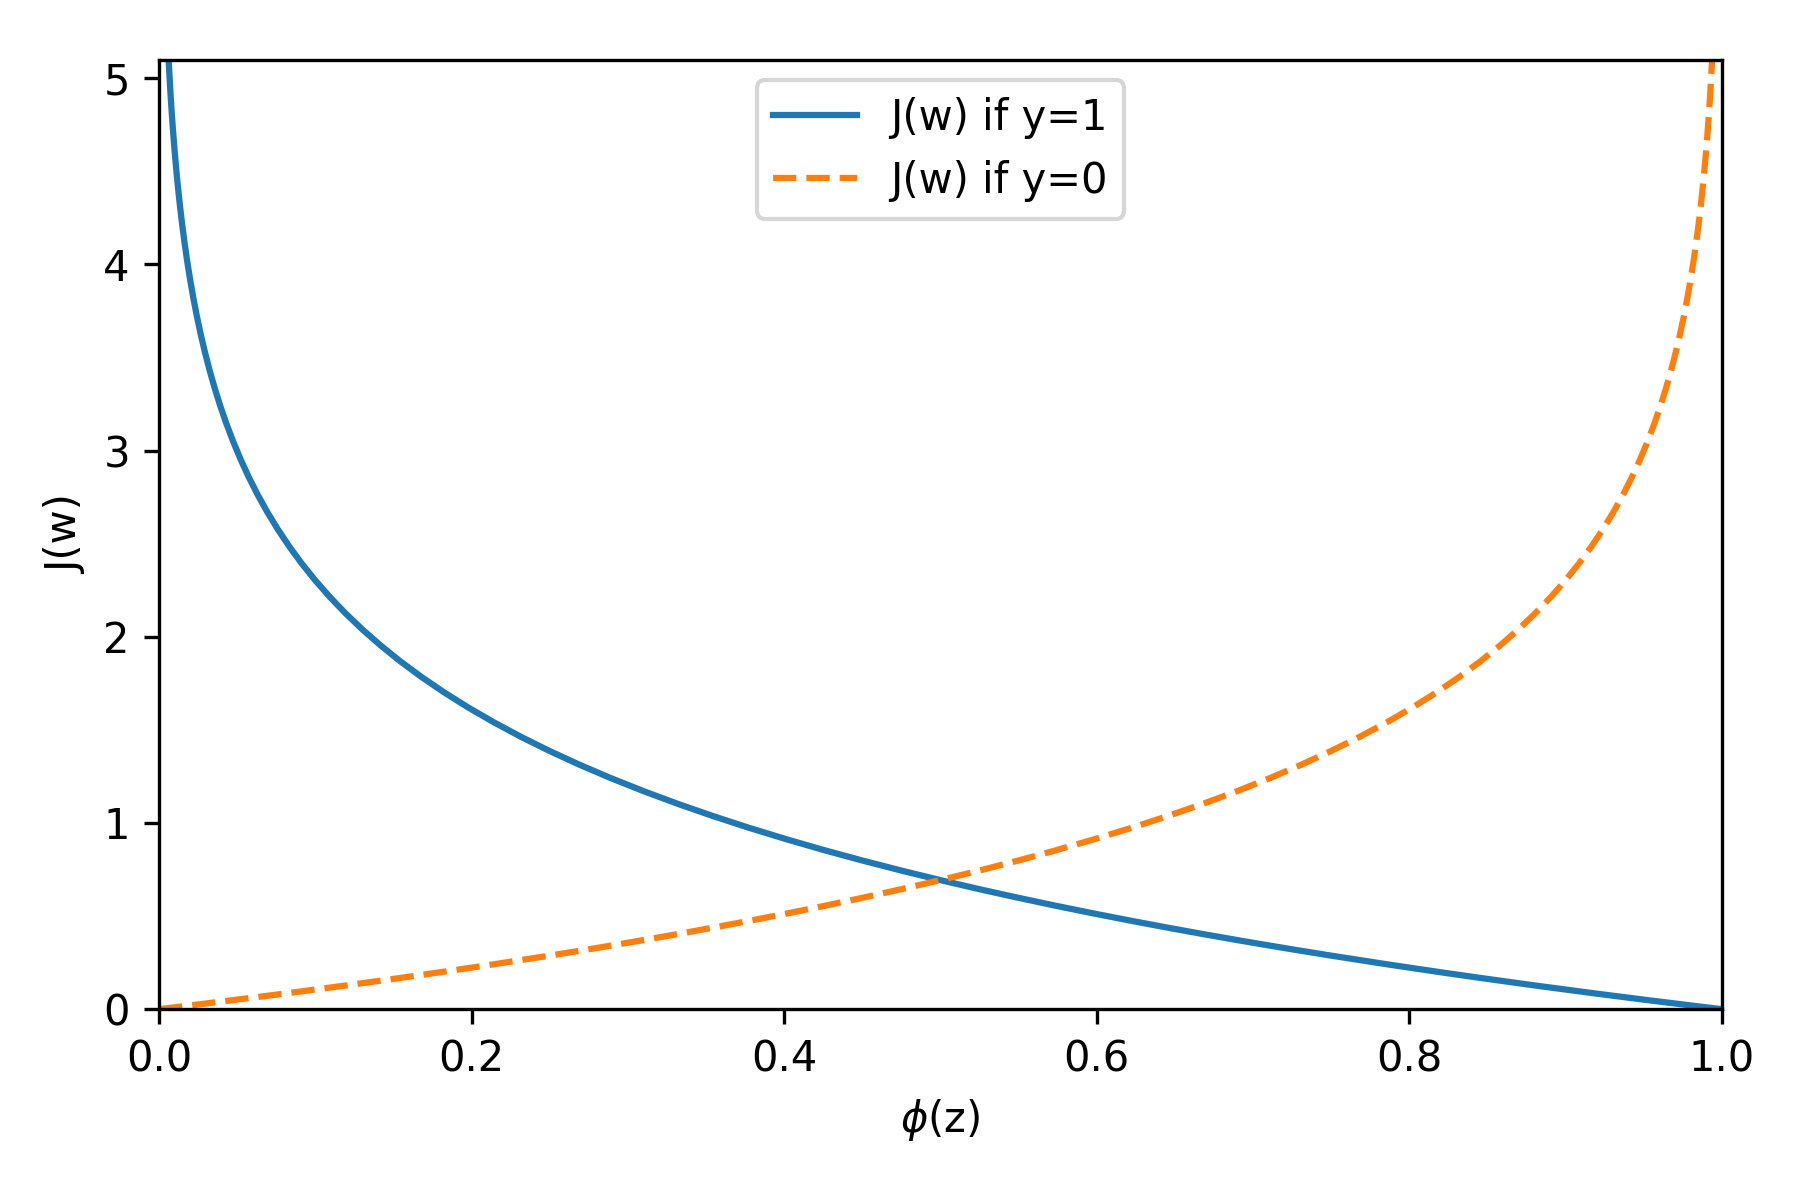
\includegraphics[width=9cm]{images/minimum_log_curve.png}
		\caption{Graphique d'une courbe de régression logistique ajustée aux données $(x_n , y_n)$. \cite[image de]{ml2008python}
		}
		\label{fig:minimum_log_curve}
	\end{figure}
	
	
	
	
	\section{Descente de gradient stochastique}
	Cette section est inspirée des articles écrites par Léon Bottou et al, dans  \cite{bottou2012stochastic} 
	\cite{bottou2010large}
	\cite{framling2004scaled}
	\cite{bottou2018optimization}
	\cite{netrapalli2019stochastic}
	\cite{wijnhoven2010fast}.
	
	\subsection{Descente de gradient (Gradient Descent)}
	
	
	Il a souvent été proposé de minimiser le risque empirique [E] en utilisant la descente de gradient (GD). Chaque itération met à jour les poids w en fonction du gradient de [E] \cite{bottou2012stochastic}.\\
	
	\lipsum[1] \\ 
	
	$$A = \begin{pmatrix}
		x_{11} & x_{12} & x_{13} & \cdots & x_{1n} \\
		x_{21} & x_{22} & x_{23} & \cdots & x_{2n} \\
		\vdots & \vdots & \vdots & \ddots & \vdots \\
		x_{m1} & x_{m2} & x_{m3} & \cdots & x_{mn} 
	\end{pmatrix}$$
	
	
	\lipsum[4]
	\subsubsection{Pourquoi stochastique?}
	Descente de gradient stochastique (SGD) 
	
	L'algorithme de descente de gradient stochastique (SGD) est une simplification drastique. Au lieu de calculer exactement le gradient de E n (f w ), chaque itération estime ce gradient sur la base d'un seul exemple z t pris au hasard \cite{bottou2012stochastic} :
	$$
	{\displaystyle w:=w-\eta \nabla Q(w)=w-{\frac {\eta }{n}}\sum _{i=1}^{n}\nabla Q_{i}(w),}
	$$
	\lipsum[1]	
	\subsection{La convergence de la descente de gradient stochastique}
	\lipsum[1]
	\subsection{Le problème des minima locaux} \cite[page 291][]{antoine2018apprentissage}????
	
	
	\section{Retro propagation}
	
	
	\section{Les optimiseurs SGD}
	\subsection{Perceptron Optimizer}
	
	
	
	\subsection{Neurone linéaire adaptatif (ADALINE)}
	\lipsum[1]
	
	\subsection{ADAM}
